\documentclass{article}
\usepackage[utf8]{inputenc}
\usepackage{tikz}
\usepackage{graphics}
\usepackage{lipsum}
\usetikzlibrary{shapes.geometric, arrows}


% FOR Different plots and charts
\usepackage{pgfplots}
\usepackage{pgfplotstable}
\pgfplotsset{compat=newest}
\usepackage{pgf-pie}
\usepackage{csquotes}
\usepackage{bchart}

% FOR FLOW CHART DECLARATION
\tikzstyle{startstop} = [ellipse,  minimum width=3cm, minimum height=1cm,text centered, draw=black, fill=red!30]
\tikzstyle{io} = [trapezium, trapezium left angle=70, trapezium right angle=110, minimum width=3cm, minimum height=1cm, text centered, draw=black, fill=blue!30]
\tikzstyle{process} = [rectangle, minimum width=3cm, minimum height=1cm, text centered, draw=black, fill=orange!30]
\tikzstyle{decision} = [diamond, aspect=4, minimum width=3cm, minimum height=1cm, text centered, draw=black, fill=green!30]
\tikzstyle{arrow} = [thick,->,>=stealth]

% FPR IMPORTING
\pgfplotsset{compat=1.15}
\usepackage{mathrsfs}
\definecolor{zzttqq}{rgb}{0.6,0.2,0.}
\definecolor{xdxdff}{rgb}{0.49019607843137253,0.49019607843137253,1.}
\definecolor{qqttqq}{rgb}{0.,0.2,0.}
\definecolor{ududff}{rgb}{0.30196078431372547,0.30196078431372547,1.}

\title{Lecture Class on Drawing Tools}
\author{nafisit03 Tripto}
\date{May 2021}

\begin{document}

\maketitle

\section{Introduction}
\lipsum[1]


\begin{figure}[h]
    \centering
\begin{tikzpicture}
\draw (0,0) -- (4,0) -- (4,4) -- (0,4) -- cycle;
\end{tikzpicture}
    \caption{Caption}
    \label{fig:my_label}
\end{figure}

\lipsum[1]

\begin{figure}[h]
    \centering
\begin{tikzpicture}
\draw[blue, dashed] (0,0) rectangle (4,6);
\draw[red, thick] (2,2) circle (3);
\draw (0,0) parabola (4,4);
\draw[teal, xshift = 6cm, yshift = 7cm] (0,0)-- node[below] {a} (3,0)--(0,2)--cycle;
\end{tikzpicture}
    \caption{Second figure}
    \label{fig:my_label1}
\end{figure}

\subsection{Axix and Grids}
\lipsum[1]


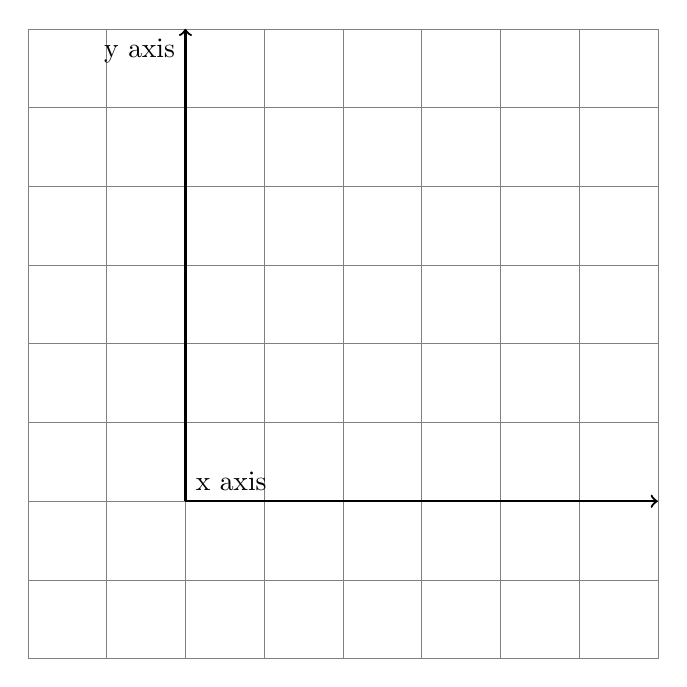
\begin{tikzpicture}
\draw[step=1cm,gray,very thin] (-2,-2) grid (6,6);
\draw[thick,->] (0,0) node[anchor = south west] {x axis}  --   (6,0) ;
\draw[thick,->] (0,0) -- (0,6) node[anchor=north east] {y axis};
\end{tikzpicture}

\section{Flow-chart}
\lipsum[1]

\begin{figure}[h]
    \centering
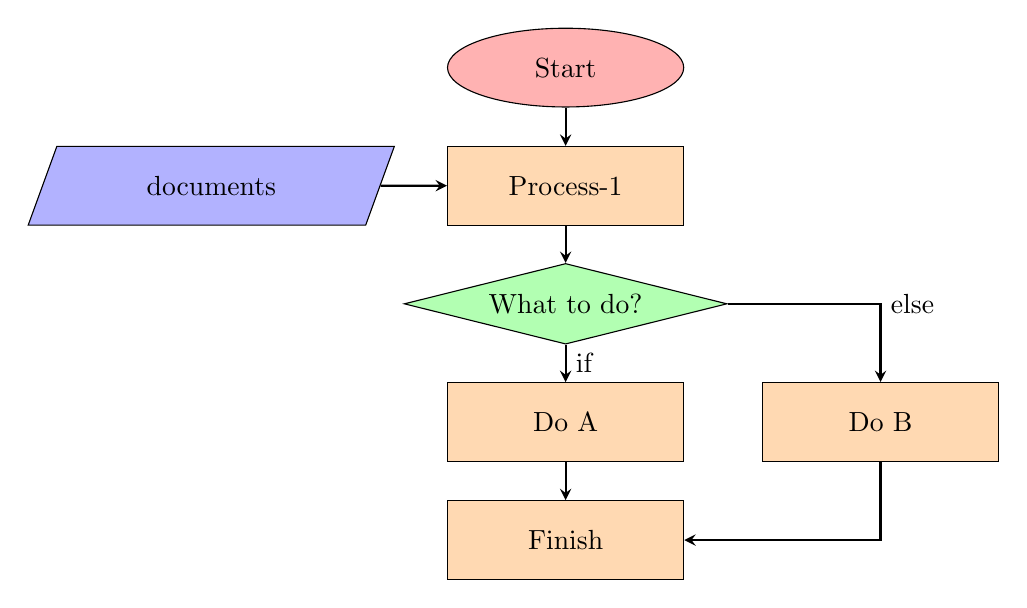
\begin{tikzpicture}

\node[startstop] (start) {Start}; 
\node[process, below of = start, yshift = -0.5cm] (p1) {Process-1};
\node[io, left of = p1, xshift = -3.5cm] (io1) {documents};
\node[decision, below of = p1, yshift=-0.5cm] (dec1) {What to do?};
\node[process, below of = dec1, yshift=-0.5cm] (p2) {Do A};
\node[process, right of = p2, xshift = 3 cm ] (p3) {Do B};
\node[process, below of = p2, yshift=-0.5cm] (end) {Finish};

\draw[arrow] (start) -- (p1);
\draw[arrow] (io1) -- (p1);
\draw[arrow] (p1) -- (dec1);
\draw[arrow] (dec1) -- node[right] {if} (p2);
\draw[arrow] (dec1) -| node[right] {else} (p3);
\draw[arrow] (p2) -- (end);
\draw[arrow] (p3) |- (end);

\end{tikzpicture}
    \caption{Flow-chart}
    \label{fig:my_label11}
\end{figure}


\section{Charts}

\subsection{Pie-chart}
\lipsum[1]

\begin{figure}[h]
    \centering
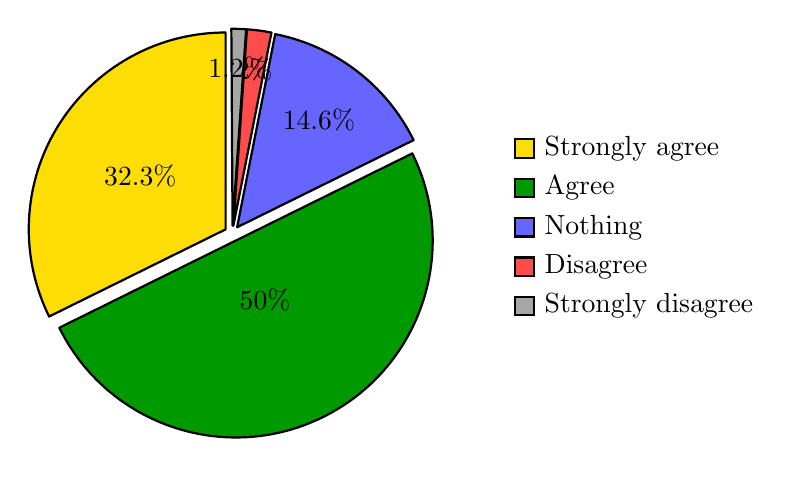
\begin{tikzpicture}

\pie[text=legend,rotate = 30,radius=2.5, rotate = 90, explode = 0.1,
color = {
        yellow!90!red,
        green!60!black,
        blue!60, red!70,
        gray!70,
        teal!20}]
  {32.3/Strongly agree,
         50/Agree,
         14.6/Nothing,
         2/Disagree,
         1.2/Strongly disagree}

\end{tikzpicture}
    \caption{Pie chart}
    \label{fig:my_label21}
\end{figure}

\subsection{bar chart}
\lipsum[1]

\begin{figure}[h]
    \centering
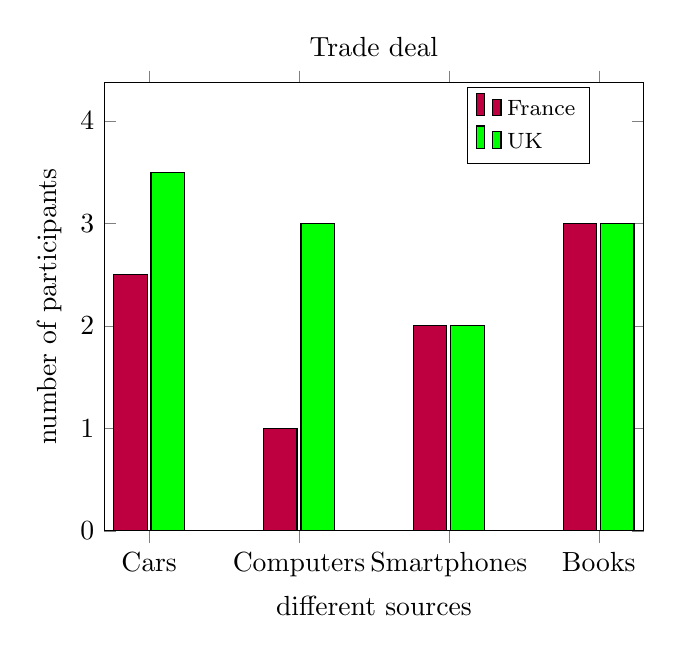
\begin{tikzpicture}

\begin{axis} [
title  = Trade deal,
ybar = .05cm,
    bar width = 12pt,
    ymin = 0,
    % ymax = 4,
    xtick = data,
    ylabel= number of participants,
    xlabel= different sources,
     legend style={at={(.9,0.99)}, font=\footnotesize, legend cell align=left,},
    enlarge y limits = {value = .25, upper},
    % enlarge x limits = {abs = 20},
    symbolic x coords = {Cars, Computers, Smartphones, Books},
    %  nodes near coords, % this command is used to mention the y-axis points on the top of the particular bar.  
    % nodes near coords align={vertical},  
]

% \addplot[fill=purple] coordinates {(1,2.5) (2,1) (3,2) (4,3)};
% \addplot[fill=green] coordinates {(1,3.5) (2,1) (3,2) (4,3)};

\addplot[fill=purple] coordinates {(Cars,2.5) (Computers,1) (Smartphones,2) (Books,3)};
\addplot[fill=green] coordinates {(Cars,3.5) (Computers,3) (Smartphones,2) (Books,3)};

\legend {France, UK};
\end{axis}


\end{tikzpicture}
    \caption{Bar chart}
    \label{fig:my_label213}
\end{figure}


\section{Direct Import}
\lipsum[1]

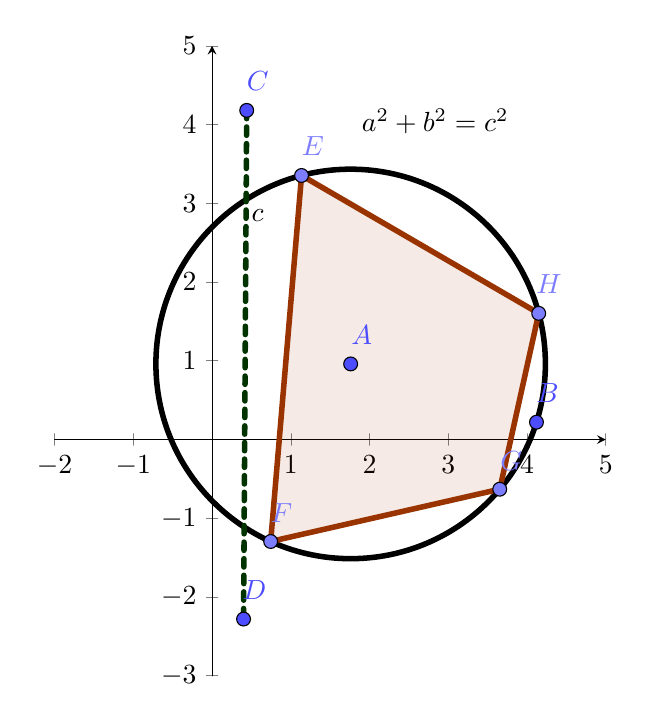
\begin{tikzpicture}[line cap=round,line join=round,>=triangle 45,x=1.0cm,y=1.0cm]
\begin{axis}[
x=1.0cm,y=1.0cm,
axis lines=middle,
xmin=-2.0,
xmax=5.0,
ymin=-3.0,
ymax=5.0,
xtick={-2.0,-1.0,...,5.0},
ytick={-3.0,-2.0,...,5.0},]
\clip(-2.,-3.) rectangle (5.,5.);
\fill[line width=2.pt,color=zzttqq,fill=zzttqq,fill opacity=0.10000000149011612] (1.1365043657105163,3.3534187251757595) -- (0.7442014451668675,-1.2950727917295537) -- (3.6534189793735257,-0.63127765287775) -- (4.148448619784679,1.6022718977572246) -- cycle;
\draw [line width=2.pt] (1.76,0.96) circle (2.4732973941683607cm);
\draw [line width=2.pt,dash pattern=on 3pt off 3pt,color=qqttqq] (0.44,4.18)-- (0.4,-2.28);
\draw [line width=2.pt,color=zzttqq] (1.1365043657105163,3.3534187251757595)-- (0.7442014451668675,-1.2950727917295537);
\draw [line width=2.pt,color=zzttqq] (0.7442014451668675,-1.2950727917295537)-- (3.6534189793735257,-0.63127765287775);
\draw [line width=2.pt,color=zzttqq] (3.6534189793735257,-0.63127765287775)-- (4.148448619784679,1.6022718977572246);
\draw [line width=2.pt,color=zzttqq] (4.148448619784679,1.6022718977572246)-- (1.1365043657105163,3.3534187251757595);
\draw (1.78,4.32) node[anchor=north west] {$a^2 + b^2 = c^2$};
\begin{scriptsize}
\draw [fill=ududff] (1.76,0.96) circle (2.5pt);
\draw[color=ududff] (1.9,1.33) node {$A$};
\draw [fill=ududff] (4.12,0.22) circle (2.5pt);
\draw[color=ududff] (4.26,0.59) node {$B$};
\draw[color=black] (0.58,2.85) node {$c$};
\draw [fill=ududff] (0.44,4.18) circle (2.5pt);
\draw[color=ududff] (0.58,4.55) node {$C$};
\draw [fill=ududff] (0.4,-2.28) circle (2.5pt);
\draw[color=ududff] (0.54,-1.91) node {$D$};
\draw [fill=xdxdff] (1.1365043657105163,3.3534187251757595) circle (2.5pt);
\draw[color=xdxdff] (1.28,3.73) node {$E$};
\draw [fill=xdxdff] (0.7442014451668675,-1.2950727917295537) circle (2.5pt);
\draw[color=xdxdff] (0.88,-0.93) node {$F$};
\draw [fill=xdxdff] (3.6534189793735257,-0.63127765287775) circle (2.5pt);
\draw[color=xdxdff] (3.8,-0.27) node {$G$};
\draw [fill=xdxdff] (4.148448619784679,1.6022718977572246) circle (2.5pt);
\draw[color=xdxdff] (4.28,1.97) node {$H$};
\end{scriptsize}
\end{axis}
\end{tikzpicture}


\end{document}
